\documentclass[11pt]{article}

\usepackage{fullpage} 
\usepackage{hyperref}
\usepackage{amsmath}
\usepackage{amssymb}
\usepackage{amsthm}
\usepackage{graphicx}
\usepackage{pgf}
\usepackage{tikz}
\usepackage{longtable}
\usepackage{wasysym}
\usepackage{enumitem}
\usepackage{xcolor}
\usepackage{color, colortbl}
\usepackage{longtable}
\usepackage{datetime}


\usetikzlibrary{arrows,automata}

\usepackage{indentfirst}

\newcommand{\question}[2] {\vspace{0.3in}\noindent{\subsection*{Question #1. #2} \vspace{0.15in}}}

\renewcommand{\part}[1] {{\vspace{0.15in}\noindent\textbf (#1)} \vspace{0.10in}}

\definecolor{dark-blue}{RGB}{23,20,119}
\definecolor{dark-green}{RGB}{2,101,15}
\definecolor{tableheadcolor}{gray}{0.65}
\definecolor{tablerowcolor}{gray}{0.90} 



%  ----------------------------------------------------------------
%                         Start here
% ----------------------------------------------------------------
 
\begin{document}

\title{Assignment \#5} %Replace X with the appropriate number
\author{\Large Gustavo Estrela de Matos\\ %Replace with your name
CSCE 433: Formal Languages and Automata} %If necessary, replace with your course number and title
\date{\today} 

\maketitle

\question{1}{}  
\begin{itemize}
\item{Eliminate the starting symbol from the right hand side}
\item{Eliminate $\epsilon$ rules}
\begin{equation*}
\begin{aligned}
    S & \rightarrow AB \mid aB \mid B \\
    A & \rightarrow aab \\
    B & \rightarrow bbA \mid bb
\end{aligned}
\end{equation*}
\item{Eliminate unity rules}
\begin{equation*}
\begin{aligned}
    S & \rightarrow AB \mid aB \mid bbA \mid bb \\
    A & \rightarrow aab \\
    B & \rightarrow bbA \mid bb 
\end{aligned}
\end{equation*}
\item{Eliminate rules with more than 2 symbols in the right hand side}
\begin{equation*}
\begin{aligned}
    S & \rightarrow AB \mid aB \mid bY \mid bb \\  
    A & \rightarrow aZ \\
    B & \rightarrow bY \mid bb \\
    Y & \rightarrow bA \\
    Z & \rightarrow ab 
\end{aligned}
\end{equation*}
\item{Create unity rules for terminals}
\begin{equation*}
\begin{aligned}
    S & \rightarrow AB \mid XB \mid VY \mid VV \\  
    A & \rightarrow XZ \\
    B & \rightarrow VY \mid VV \\
    Y & \rightarrow VA \\
    Z & \rightarrow VX \\
    V & \rightarrow b \\
    X & \rightarrow a
\end{aligned}
\end{equation*}
\end{itemize}

\question{2}{}
\part{a} \\
\begin{figure}[h]
\centering
\fbox{
    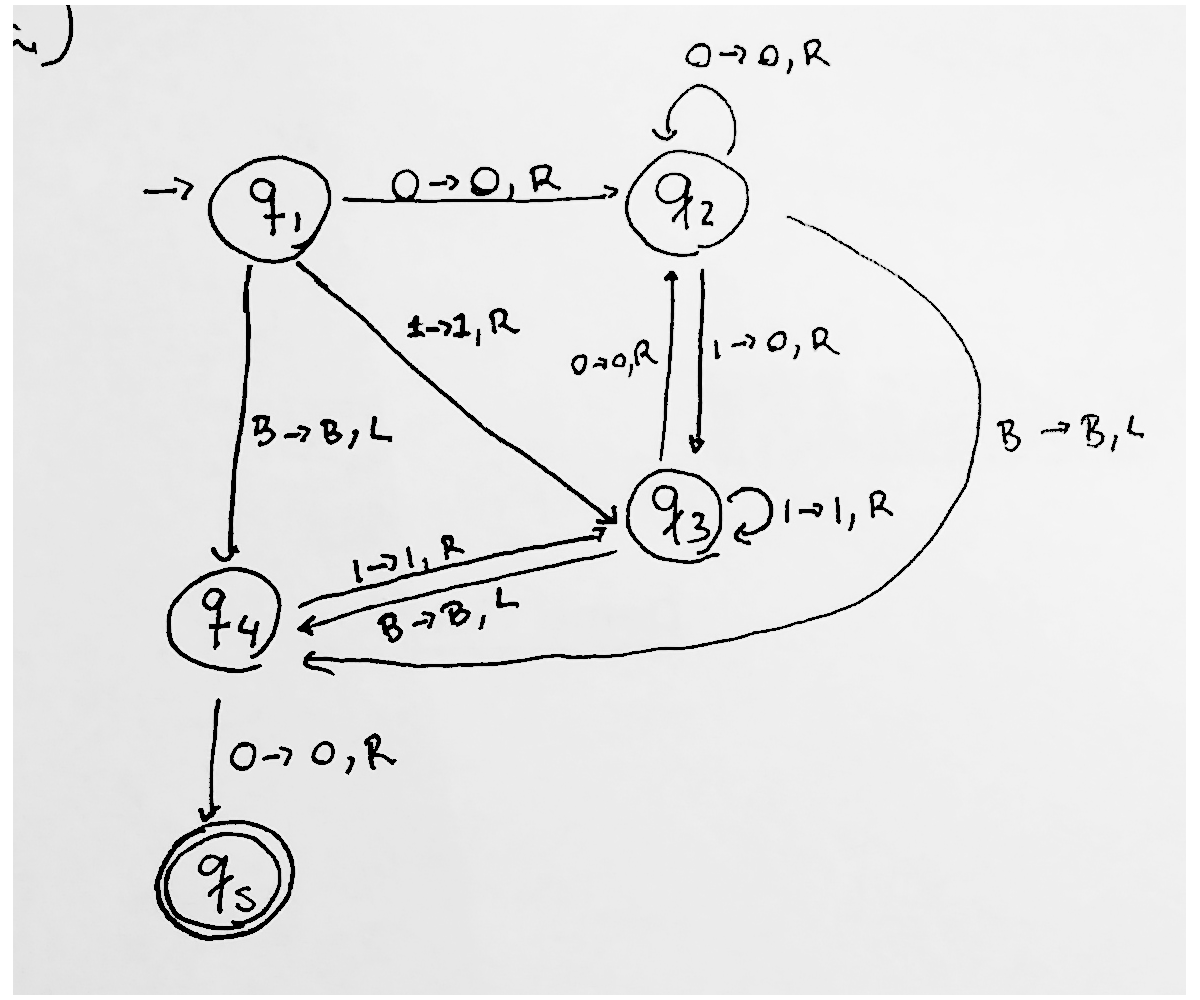
\includegraphics[scale=.2]{2a.png}
}
\end{figure}

\part{b} \\
$q_100110 \vdash$
$0q_20110 \vdash$
$00q_2110 \vdash$
$000q_310 \vdash$
$0001q_30 \vdash$
$00010q_2 \vdash$
$0001q_40 \vdash$
$00010q_5$ \\
\part{c} \\
$q_1111010 \vdash$
$1q_311010 \vdash$
$11q_31010 \vdash$
$111q_3010 \vdash$
$1110q_210 \vdash$
$11100q_30 \vdash$
$111000q_2 \vdash$
$11100q_40 \vdash$
$111000q_5$

\question{3}{}
\part{a} \\

\par The idea implemented in this TM is to match a's from left to right (replacing with A's) with the c's from right to left, and when this is done it should match b's from left to right with the A's from right to left. \\
\begin{figure}[h]
\centering
\fbox{
    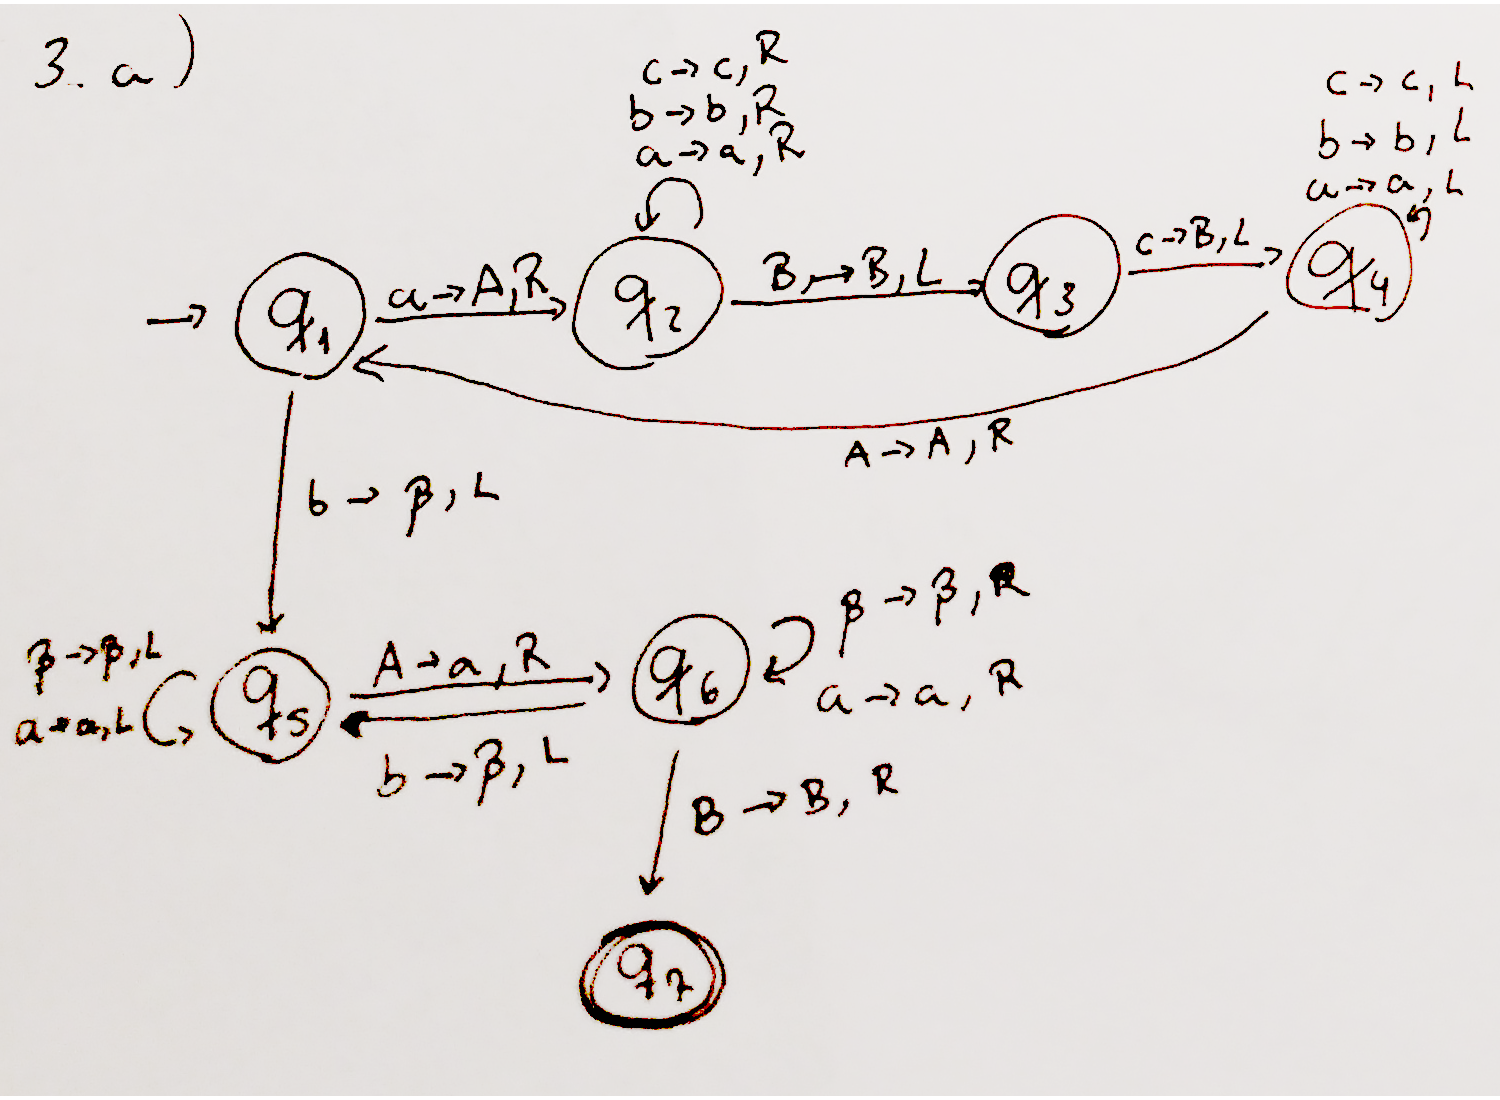
\includegraphics[scale=.2]{3a.png}
}
\end{figure}
\newpage

\part{b} \\
\par We can split this machine in two other problems. First we divide the string in the middle, then we match every character of the two produced strings. To divide the string in two we are going to shift left the beggining of the string and the shift right the end of the string until the symbols we use for keeping track of the shifting meet in the middle of the first string. The second part is basically going to the beggining of the two strings and comparing the symbols.
\begin{figure}[h]
\centering
\fbox{
    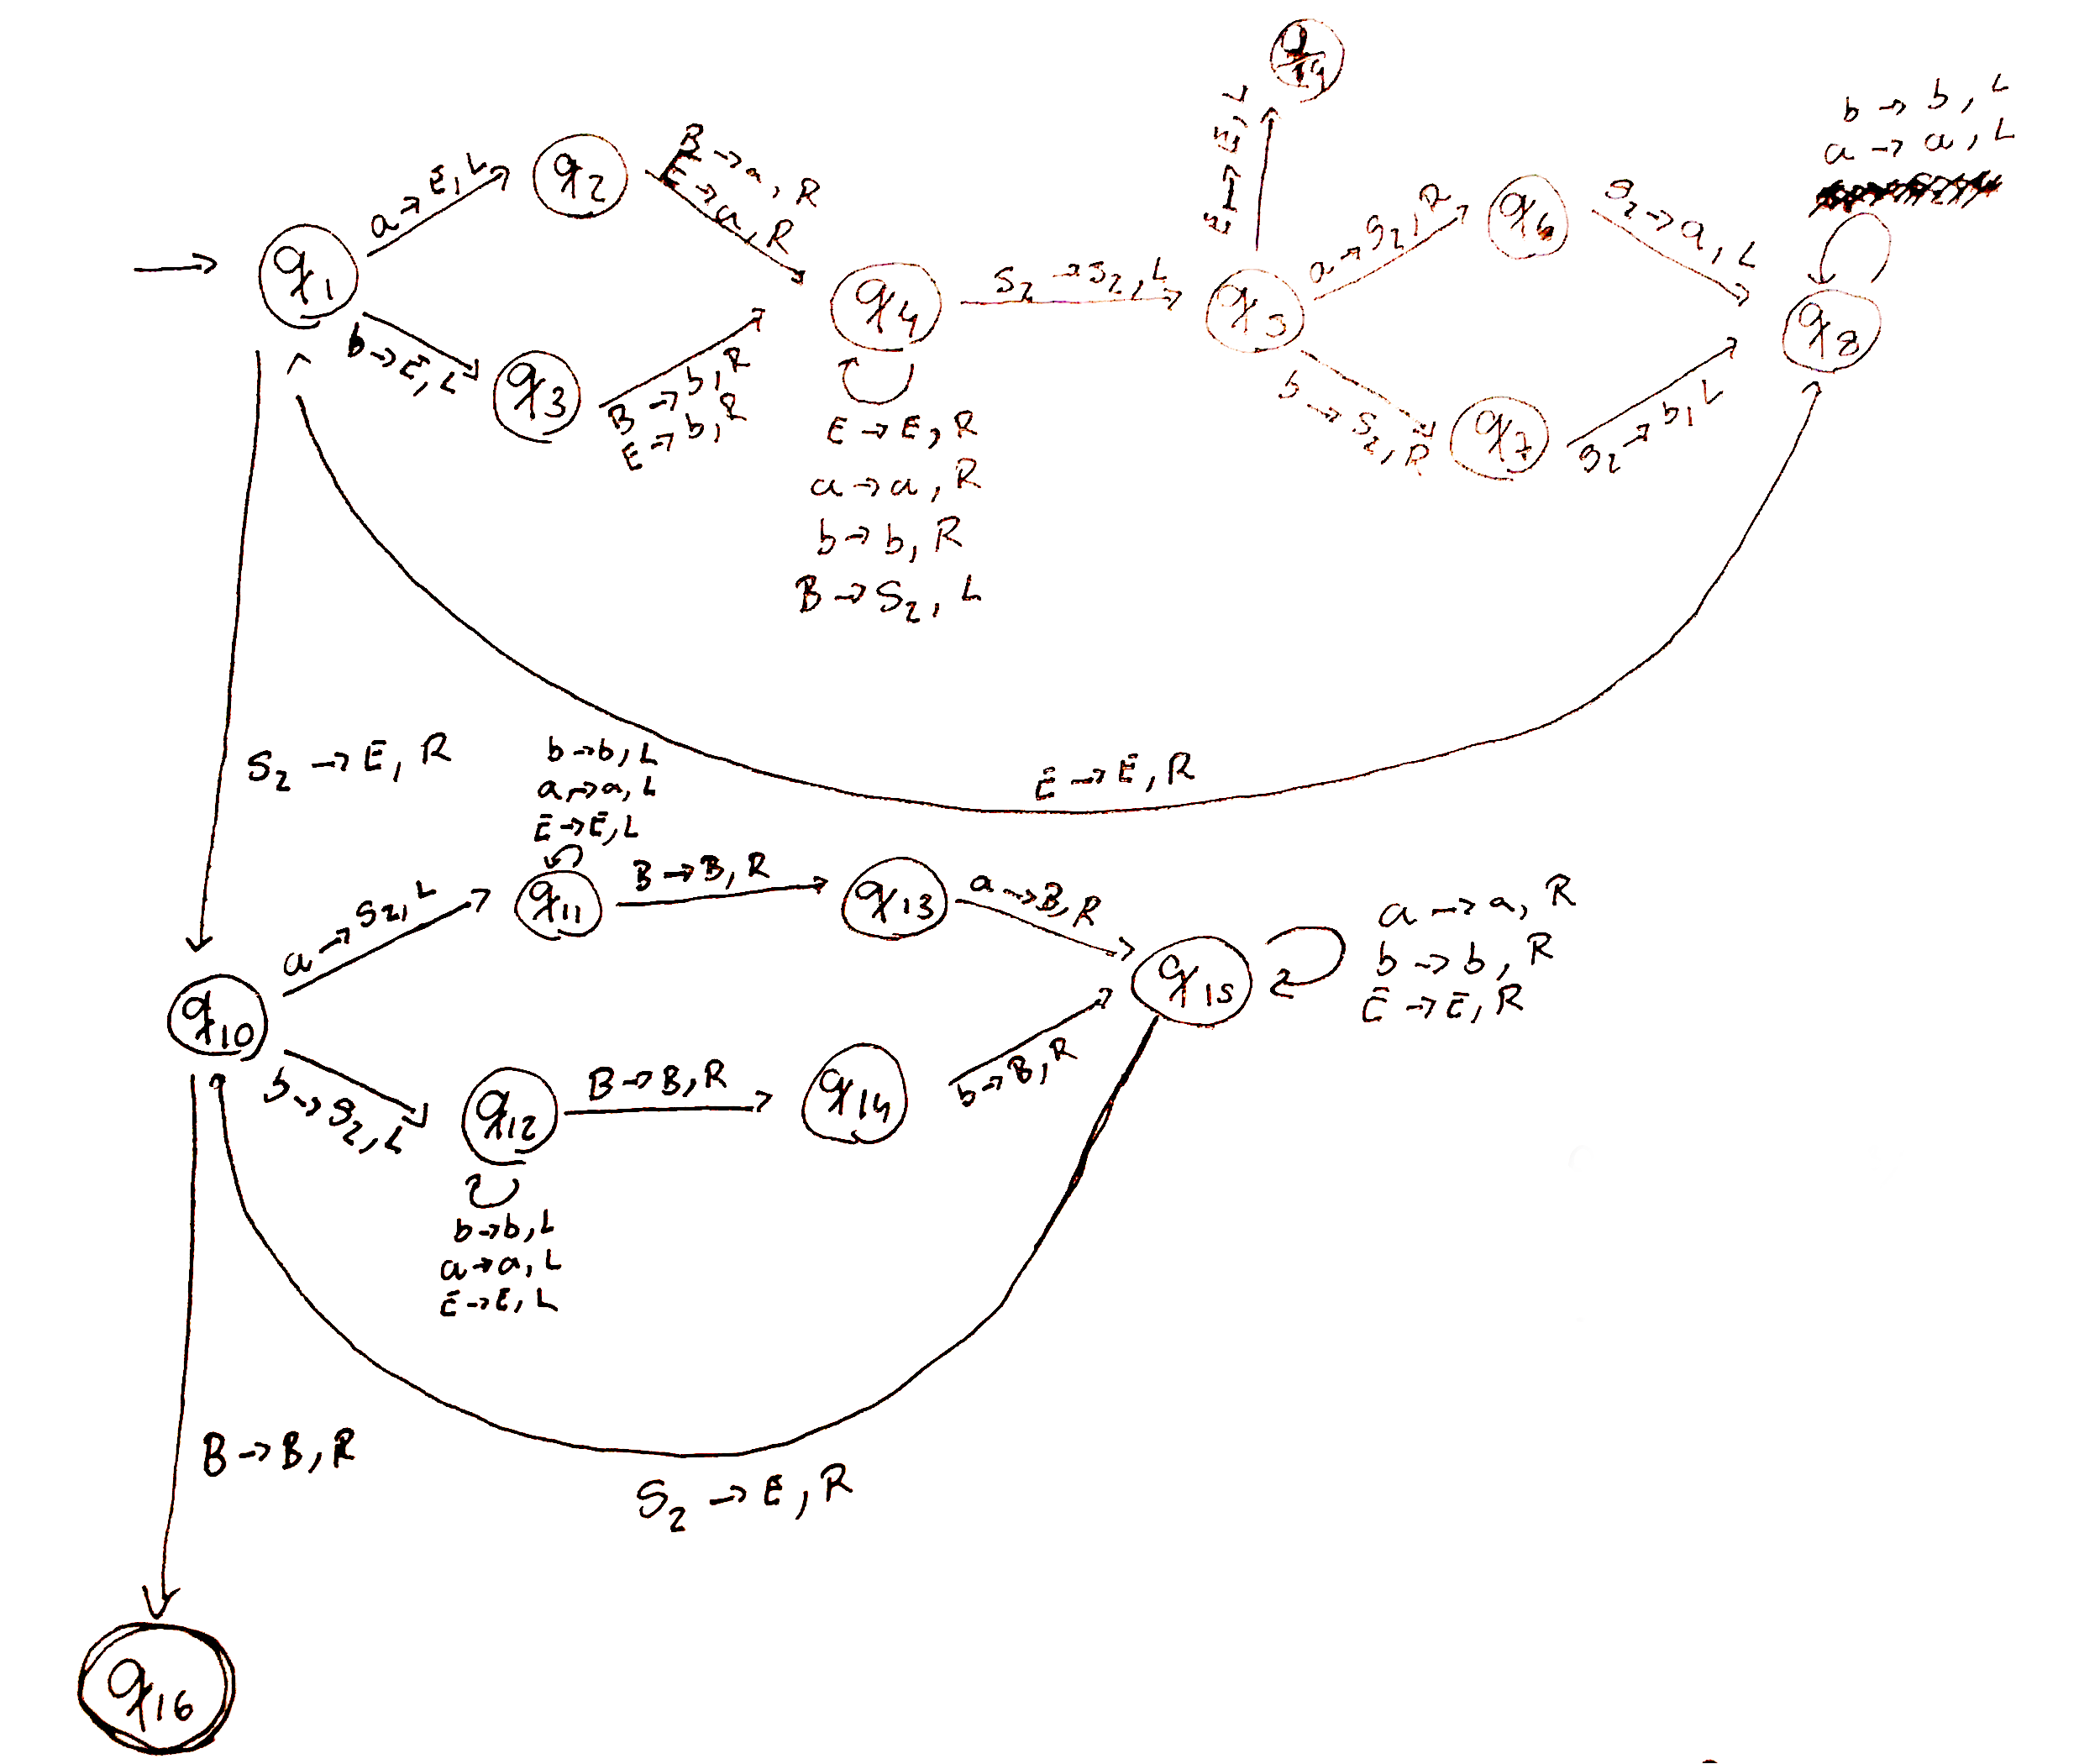
\includegraphics[scale=.1]{3b.png}
}
\end{figure}
\newpage

\question{4}{}
\par This machine does the algorithm we normally do by hand, from right to left, bit by bit. The key idea is that we are summing $N$ with $0$ and starting the carry with $1$. The carry is $1$ when we are in the state $q_1$ and it is $0$ when we are in the state $q_2$.
\begin{figure}[h]
\centering
\fbox{
    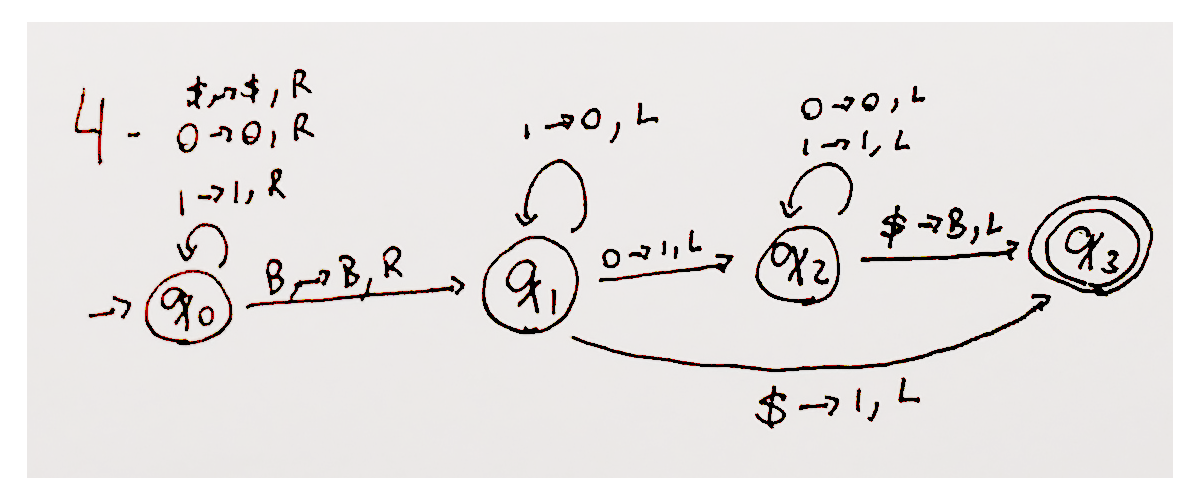
\includegraphics[scale=.2]{4.png}
}
\end{figure}


\question{5}{}
\par As we saw in class, the symbol $w_i$ is such that $1w_i = i_2$. Therefore, since $37 = (100101_2)$ we have that $1w_{37} = 100101$ and $w_{37} = 00101$.

\question{6}{}
\begin{itemize}
    \item{Transitions code:}
    \begin{equation*}
    \begin{aligned}
        \delta (q_1, 0) = (q_3, 0, R) & & C_1 = 01010001010 \\
        \delta (q_1, 1) = (q_5, 1, R) & & C_2 = 010010000010010 \\
        \delta (q_1, B) = (q_5, B, L) & & C_3 = 010001000001000100 \\
        \delta (q_3, 0) = (q_3, 0, R) & & C_4 = 0001010001010 \\
        \delta (q_3, 1) = (q_4, 0, R) & & C_5 = 000100100001010 \\
        \delta (q_3, B) = (q_5, B, L) & & C_6 = 00010001000001000100 \\
        \delta (q_4, 0) = (q_3, 0, R) & & C_7 = 00001010001010 \\
        \delta (q_4, 1) = (q_4, 1, R) & & C_8 = 00001001000010010 \\
        \delta (q_4, B) = (q_5, B, L) & & C_9 = 000010001000001000100 \\
        \delta (q_5, 0) = (q_2, 0, R) & & C_{10} = 00000101001010 \\
        \delta (q_5, 1) = (q_4, 1, R) & & C_{11} = 000001001000010010 
    \end{aligned}
    \end{equation*}
    \item{The machine code: } \\
        $C_1 11 C_2 11 C_3 11 C_4 11 C_5 11 C_6 11 C_7 11 C_8 11 C_9 11 C_{10} 11 C_{11}$
\end{itemize}

\question{7}{}
\part{a} \\
\par $L$ is CFL. First, we prove that it's not regular using the Pumping Lemma. Assume that $L$ is regular with pumping constant $p$ and consider the string $s = a^pb^{2p}a^p \in L$. Accoding to the Pumping Lemma, we can write $s = xyz$ where $|xy| \leq p$ and $|y| \geq 1$, and also $s' = xy^0z$ should be in $L$. Since $|xy| \leq p$ we have that $y = a^i$, therefore $s' = a^{p - i}b^{2p}a^p$ and this string should not be in $L$ because $s' \neq reverse(s')$, which contradicts the pumping lemma. Since we have a contradiction, we conclude that our assumption is false and $L$ is not regular.
\par To prove that this language is a Context Free Language we can construct a grammar for it: $S \rightarrow \epsilon \mid aaSaa \mid baSab \mid abSba \mid bbSbb$.

\part{b} \\
\par $\overline L$ is CFL. First we prove that it's not regular using closure properties. Assume that $\overline L$ is regular, then $L$ should also be regular. Note that $L = \{w \mid w = reverse (w)$ and $|w|$ is divisible by $2\}$, therefore $L \cap ((a+b)(a+b)(a+b)(a+b))^*$ is regular and is the same as $\{w \mid w = reverse (w)$ and $|w|$ is divisible by $4\}$, the language that we proved in $a)$ that is not regular, a contradiction. Therefore the assumption that $\overline L$ is regular is false.

\par We show that $\overline L$ is regular by building a PDA. This PDA accepts either strings with odd size or strings with even size but not in the format $ww^R$
\begin{figure}[h]
\centering
\fbox{
    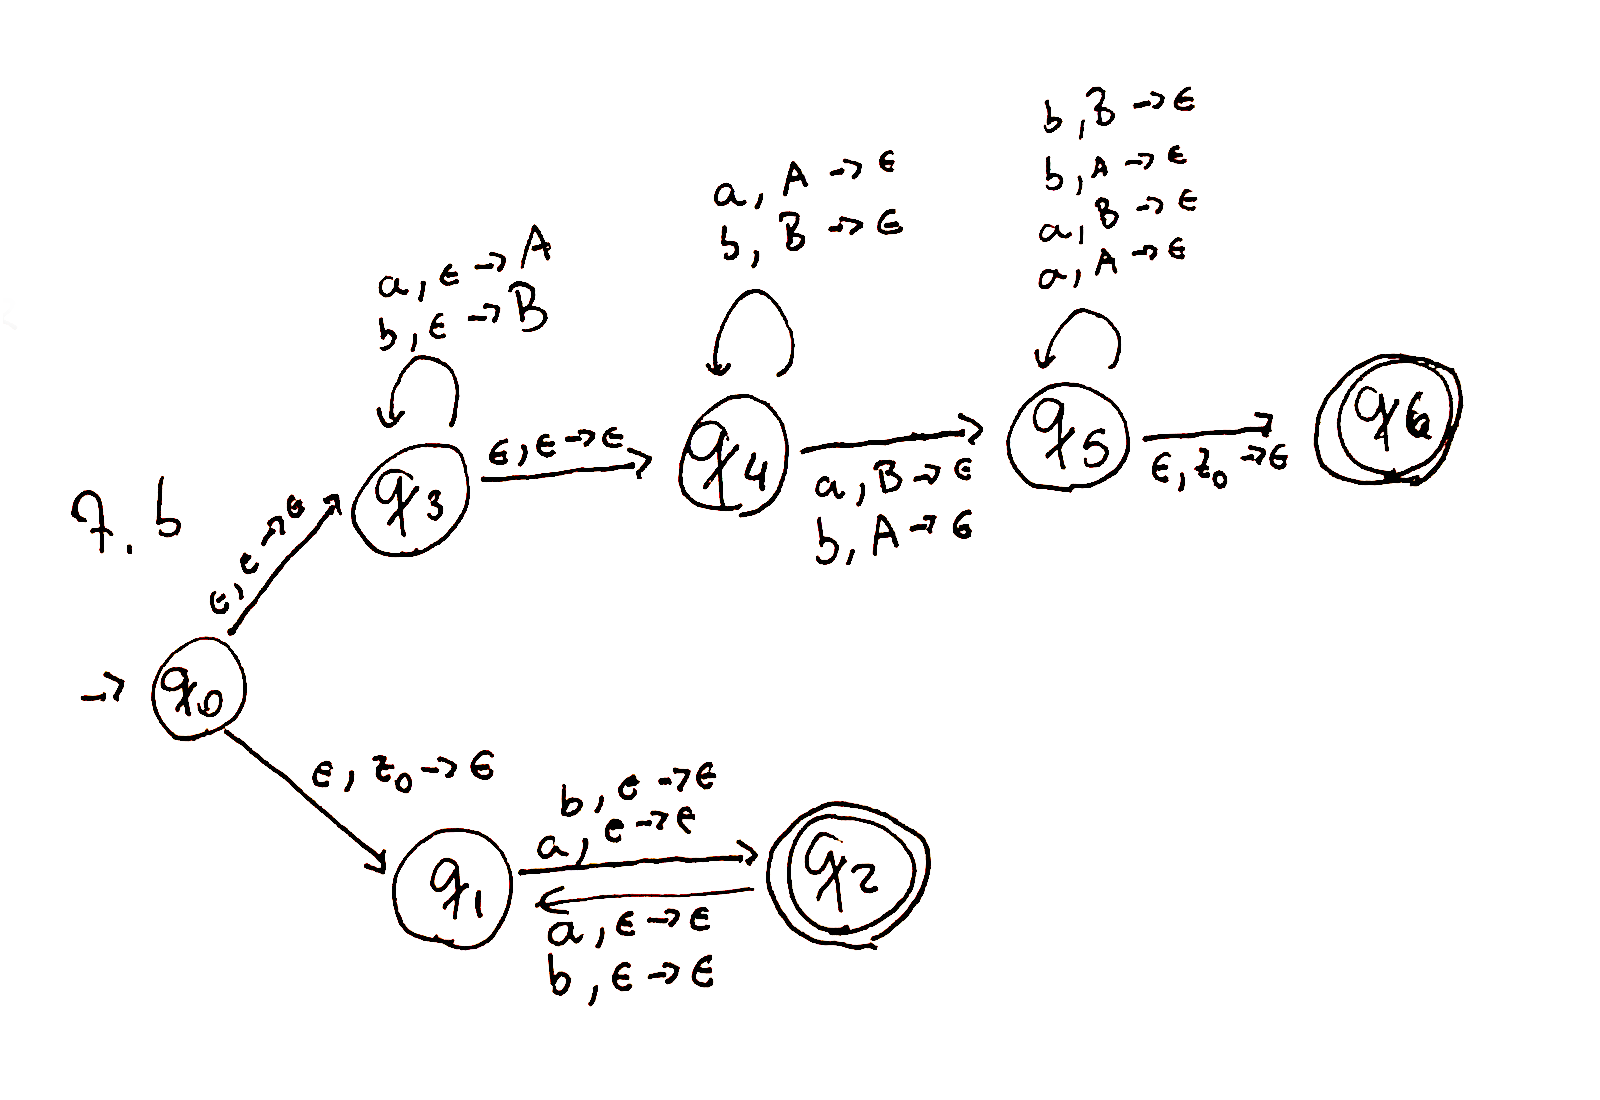
\includegraphics[scale=.2]{7b.png}
}
\end{figure}



\part{c} \\
$L$ is regular. We prove this by giving a regular expression for this language: $(b^*ab^*ab^*ab^*ab^*)^*ab^*$
\end{document}
